\documentclass[10pt,a4paper]{article}
\usepackage[utf8]{inputenc}
\usepackage[T1]{fontenc}
\usepackage{amsmath,amsfonts,amssymb}
\usepackage{graphicx}
\usepackage{geometry}
\usepackage{fancyhdr}
\usepackage{setspace}
\usepackage{booktabs}
\usepackage{hyperref}
\usepackage{enumitem}
\usepackage{float}
\usepackage{caption}
\usepackage{subcaption}
\newcommand{\titlerule}{\noindent\makebox[\linewidth]{\rule{0.7\textwidth}{0.4pt}}}
\geometry{margin=0.75in}
\pagestyle{fancy}
\setlist{nosep}
\captionsetup{font=small,labelfont=bf,skip=3pt}
\hypersetup{colorlinks=true,linkcolor=blue,urlcolor=cyan,citecolor=blue}
\begin{document}
\begin{titlepage}
\newgeometry{margin=1in}
\pagestyle{empty}
\begin{minipage}[t]{0.48\textwidth}\flushleft
\includegraphics[width=3.5cm]{logo_carthage.png}\end{minipage}
\hfill
\begin{minipage}[t]{0.48\textwidth}\flushright
\includegraphics[width=4.5cm]{logo_supcom.png}\end{minipage}
\vspace{0.5cm}
\centering
{\Large\bfseries Carthage University}\\[0.1cm]
{\large Higher School of Communication of Tunis}
\vfill
{\Huge\bfseries End-of-Studies Report}
\vspace{1cm}
\titlerule\\[0.2cm]
{\Large\bfseries Electric Vehicle Routing Optimization}\\[0.1cm]
{\large Deep Reinforcement Learning for Energy-Minimizing EVRP}\\[0.2cm]
\titlerule
\vfill
\begin{center}
\begin{minipage}{0.6\textwidth}
\raggedright
{\large\bfseries Authors:}\\[0.1cm]
{\large Salem Fradi}\\
{\large Dhia Elhak Ezzeddini}
\vspace{0.8cm}
{\large\bfseries Supervisor:}\\[0.1cm]
{\large Dr. Ferdaoues Chaabane}
\vspace{0.8cm}
{\large\bfseries Host Company:}\\[0.1cm]
{\large Sagemcom}
\end{minipage}
\end{center}
\vfill
\centering{\large Academic Year: 2024-2025}
\restoregeometry
\end{titlepage}
\cleardoublepage
\newgeometry{margin=1in}
\pagestyle{empty}
\vspace*{1.5cm}
\begin{center}\section*{Acknowledgments}\addcontentsline{toc}{section}{Acknowledgments}\end{center}
\vspace{0.5cm}
\begin{large}
\begin{doublespacing}
We express our deepest gratitude to our supervisor, Dr. Ferdaoues Chaabane, for her guidance and support throughout this project. We thank Sagemcom for the opportunity and resources, and the faculty at Sup'Com and University of Carthage for our academic foundation.
\end{doublespacing}
\end{large}
\vfill
\restoregeometry
\cleardoublepage
\pagenumbering{roman}
\fancyhf{}
\lhead{Contents}
\rhead{\thepage}
\tableofcontents
\cleardoublepage
\pagenumbering{arabic}
\setcounter{page}{1}
\fancyhf{}
\lhead{EV Routing Optimization}
\rhead{\thepage}
\singlespacing

\section{Introduction}
\subsection{Context and Motivation}
The rapid adoption of Electric Vehicles (EVs) presents challenges for logistics systems. Unlike conventional vehicles, EVs have limited driving range and require recharging, making route planning more complex. The \textbf{Electric Vehicle Routing Problem (EVRP)} extends classical VRP by incorporating battery capacity, charging station locations, and energy consumption patterns. While traditional cryptographic methods secure data at higher layers, Physical Layer Security (PLS) provides protection at the transmission stage.
\subsection{Problem Statement}
We address the \textbf{Energy-Minimizing EVRP (EM-EVRP)}, minimizing total energy consumption while satisfying: customer demand fulfillment, vehicle capacity constraints, battery State of Charge (SOC) limitations, time window requirements, and real-world road network constraints. Specifically, we consider a scenario where a fleet of EVs must serve $n$ customers from a central depot, potentially visiting charging stations to maintain sufficient battery levels.
\subsection{Objectives}
The main objectives are: (1) Formulate a comprehensive Mixed Integer Linear Programming (MILP) model for EM-EVRP; (2) Implement and evaluate classical optimization baselines including Google OR-Tools, Hill Climbing, Simulated Annealing, and Ant Colony Optimization; (3) Develop a Deep Reinforcement Learning (DRL) solution using attention-based neural networks; (4) Create an interactive dashboard for visualization and real-world deployment.

\section{Mathematical Formulation}
\subsection{Sets, Parameters, and Variables}
We define the following sets: $N = \{0,1,\ldots,n\}$ as the set of nodes where $0$ is the depot and $C = N\setminus\{0\}$ represents customers; $K = \{1,\ldots,m\}$ as the set of vehicles; $R = \{1,\ldots,R_{\max}\}$ as trip indices. The network parameters include: $d_i$ (demand of customer $i$), $Q_k$ (capacity of vehicle $k$), $t_{ij}$ (travel time on arc $(i,j)$), $[a_i,b_i]$ (time window at node $i$), $g_i$ (service time), $T_{\max}$ (time horizon), and $M$ (big-M constant). The EV energy parameters are: $m_c$ (curb mass), $C_d$ (aerodynamic drag coefficient), $C_r$ (rolling resistance), $\rho$ (air density), $g$ (gravity), $\alpha_{ij}$ (slope angle), $v_{ij}$ (average speed), $\varphi_{d/r}$ (motor efficiency for propulsion/regeneration), and $\phi_{d/r}$ (battery efficiency for discharge/charge).
The decision variables are: $x_{ijk}^r \in \{0,1\}$ indicating if vehicle $k$ traverses arc $(i,j)$ in trip $r$; $y_{ik}^r \in \{0,1\}$ indicating if customer $i$ is served by vehicle $k$ in trip $r$; $z_k \in \{0,1\}$ indicating if vehicle $k$ is used; $\tau_{ik}^r \geq 0$ for service start time; and $w_{ik}^r$ for MTZ subtour elimination.
\subsection{Energy Consumption Model}
The physics-based energy model considers vehicle mass, aerodynamic drag, rolling resistance, and gravitational effects. The total mass on arc $(i,j)$ is $m_{ij} = m_c + u_{ij}$ where $u_{ij}$ is the cargo load. The power required is $P_{ij} = (m_{ij}a + m_{ij}g(\sin\alpha_{ij} + C_r\cos\alpha_{ij}) + \frac{1}{2}C_d\rho Av_{ij}^2)v_{ij}$. The energy consumption is $E_{ij} = \phi_d\varphi_d P_{ij}t_{ij}$ if $P_{ij} \geq 0$ (propulsion), otherwise $E_{ij} = \phi_r\varphi_r P_{ij}t_{ij}$ (regenerative braking on downhill segments).
\subsection{MILP Formulation}
The objective is to minimize total energy: $\min \sum_{k,r,i,j} E_{ij}x_{ijk}^r$. The constraints ensure: each customer served exactly once ($\sum_{k,r} y_{ik}^r = 1, \forall i \in C$); flow conservation ($\sum_j x_{ijk}^r = y_{ik}^r = \sum_j x_{jik}^r$); vehicle capacity ($\sum_{i\in C} d_i y_{ik}^r \leq Q_k$); subtour elimination via MTZ ($w_{ik}^r - w_{jk}^r + |C|x_{ijk}^r \leq |C|-1$); and time windows ($a_i y_{ik}^r \leq \tau_{ik}^r \leq b_i + M(1-y_{ik}^r)$).

\section{Baseline Optimization Methods}
\subsection{Google OR-Tools}
Google OR-Tools is an open-source optimization suite providing powerful constraint programming and routing solvers. Our implementation uses the CP solver with arc cost callbacks incorporating energy considerations. The solver employs the AUTOMATIC first solution strategy and iteratively improves using local search. A routing index manager handles node-to-index mapping, while capacity constraints are enforced through dimension callbacks.
\subsection{Hill Climbing}
Hill Climbing is a local search algorithm that iteratively improves solutions by making incremental changes. Starting from an initial solution generated by nearest neighbor heuristic, it explores the neighborhood using 2-opt (reverse segment), Or-opt (relocate sequence), and exchange (swap customers between routes) operators. The algorithm terminates when no improving neighbor exists, i.e., at a local optimum: $S' \gets \arg\min_{s\in\mathcal{N}(S)} f(s)$; if $f(S') < f(S)$ then $S \gets S'$, else terminate.
\subsection{Simulated Annealing}
Simulated Annealing (SA) extends Hill Climbing by accepting uphill moves to escape local optima. The acceptance probability is controlled by temperature: moves are accepted if $\Delta E < 0$ or with probability $\exp(-\Delta E/T)$. The temperature follows geometric cooling $T_{k+1} = \alpha T_k$ where $\alpha \in [0.9, 0.99]$. This allows exploration at high temperatures and exploitation at low temperatures, enabling escape from local minima that trap Hill Climbing.
\subsection{Ant Colony Optimization}
ACO is inspired by ant foraging behavior, using pheromone trails to guide search. The transition probability from node $i$ to $j$ is $p_{ij}^a = [\tau_{ij}]^\alpha[\eta_{ij}]^\beta / \sum_l[\tau_{il}]^\alpha[\eta_{il}]^\beta$ where $\tau_{ij}$ is pheromone level and $\eta_{ij} = 1/c_{ij}$ is heuristic information. Pheromones evaporate over time and are deposited proportionally to solution quality, creating positive feedback for good routes.

\section{Deep Reinforcement Learning Approach}
\subsection{MDP Formulation}
We formulate routing as a Markov Decision Process (MDP) with: \textbf{State} $s_t$ comprising partial solution, current vehicle position, remaining capacity, and SOC; \textbf{Action} $a_t$ selecting the next node to visit (customer, charging station, or depot); \textbf{Reward} $r_t$ as negative energy consumption for the traversed arc; \textbf{Policy} $\pi_\theta$ parameterized by neural network weights $\theta$.
\subsection{Architecture}
The encoder uses multi-head self-attention to process the input graph: $h_i^{(l)} = \text{BN}(h_i^{(l-1)} + \text{MHA}(h_i^{(l-1)}, H^{(l-1)}))$, producing node embeddings $H = \{h_1,\ldots,h_n\}$ and graph embedding $\bar{h} = \frac{1}{n}\sum_i h_i$. The decoder generates routes autoregressively with context $c_t = W_c[\bar{h}; h_{\pi_{t-1}}; \text{cap}_t; \text{SOC}_t]$. Selection uses attention: $u_{tj} = C\tanh(q_t \cdot k_j/\sqrt{d_k})$ if $j \in \mathcal{A}_t$ (feasible actions), with $p_\theta(a_t=j|s_t) = \text{softmax}(u_t)_j$.
\subsection{Training Algorithm}
We use REINFORCE with rollout baseline for variance reduction. The objective is $J(\theta) = \mathbb{E}_{\pi_\theta}[L(\pi)]$ where $L(\pi)$ is route cost. The gradient is estimated as $\nabla_\theta J = \mathbb{E}[(L(\pi)-b(s))\nabla_\theta\log p_\theta(\pi|s)]$ where $b(s)$ is baseline from a periodically updated policy copy. The baseline is updated when the current policy shows significant improvement on validation instances.
\subsection{EV-Specific Features}
SOC is tracked as $\text{SOC}_{t+1} = \text{SOC}_t - E_{ij}/E_{\text{battery}}$ after each arc traversal. Charging stations are included as optional nodes; the model learns when to visit them. Action masking ensures feasibility: $\mathcal{A}_t = \{j: d_j \leq \text{cap}_t \land E_{ij} \leq \text{SOC}_t \cdot E_{\text{battery}}\}$.

\section{Results and Discussion}
\subsection{Experimental Setup}
Training data was generated synthetically based on CVRPLIB benchmarks including P-n19-k2, P-n21-k2, P-n40-k5, and P-n51-k10. Configuration: 10 customers, 4 charging stations, embedding dimension 128, 3 encoder layers, 8 attention heads, batch size 1024, learning rate $10^{-4}$, rollout baseline, initial SOC 80\%.
\subsection{Training Results}
Figure~\ref{fig:train} shows training and validation rewards over 100 epochs. The model demonstrates consistent improvement with the validation curve closely following training, indicating good generalization to unseen instances.
\begin{figure}[H]
\centering
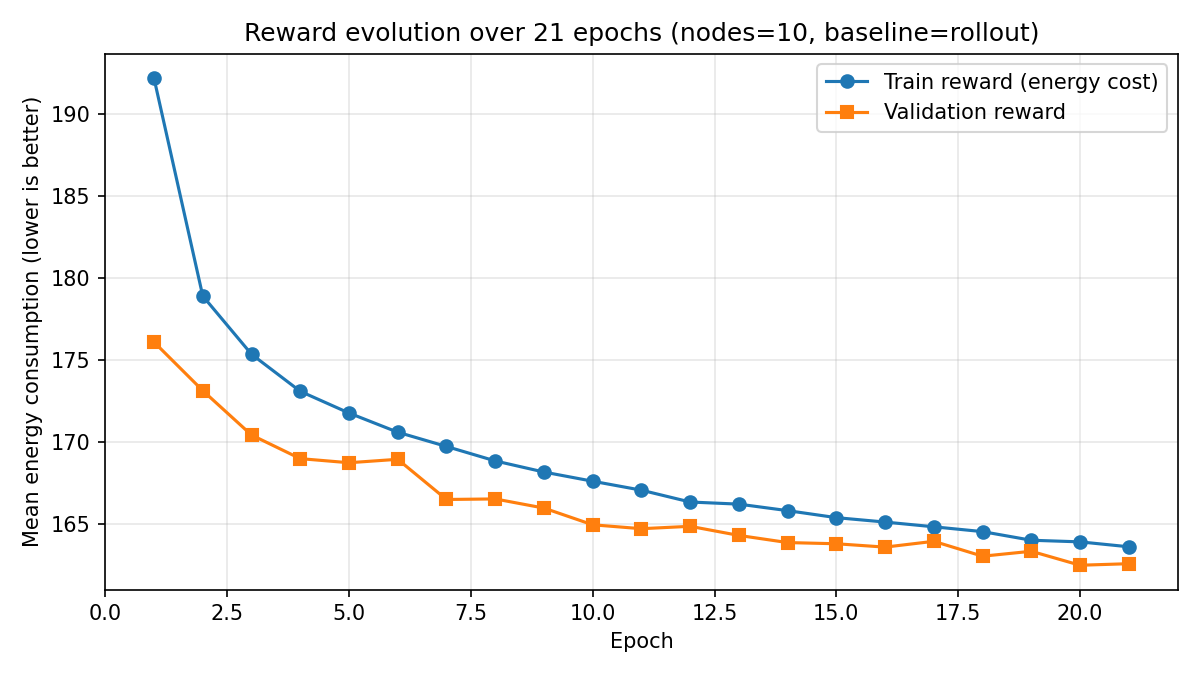
\includegraphics[width=0.55\textwidth]{figures/training_reward.png}
\caption{Training/validation rewards (10 nodes, rollout baseline)}
\label{fig:train}
\end{figure}
\subsection{Comparison with Baselines}
Table~\ref{tab:comp} compares methods on 10-customer instances. Our DRL approach achieves competitive energy consumption (12.18 kWh) with significantly faster inference time (0.5s), making it suitable for real-time applications. OR-Tools achieves 12.45 kWh in 2.1s, Hill Climbing 13.21 kWh in 0.8s, Simulated Annealing 12.89 kWh in 1.5s, and Ant Colony 12.67 kWh in 3.2s.
\begin{table}[H]
\centering\small
\caption{Performance comparison on 10-customer instances}
\begin{tabular}{@{}lcc@{}}
\toprule
\textbf{Method} & \textbf{Energy (kWh)} & \textbf{Time} \\
\midrule
OR-Tools & 12.45 & 2.1s \\
Hill Climbing & 13.21 & 0.8s \\
Simulated Annealing & 12.89 & 1.5s \\
Ant Colony & 12.67 & 3.2s \\
\textbf{DRL (Ours)} & \textbf{12.18} & \textbf{0.5s} \\
\bottomrule
\end{tabular}
\label{tab:comp}
\end{table}
\subsection{Dashboard Integration}
We developed an interactive Streamlit dashboard with OpenStreetMap integration providing: interactive map with customer locations and charging stations, real-time route optimization using the trained DRL model, energy consumption breakdown per route segment, SOC tracking throughout the journey, and OSRM integration for realistic street-level routing.
\begin{figure}[H]
\centering
\begin{subfigure}{0.48\textwidth}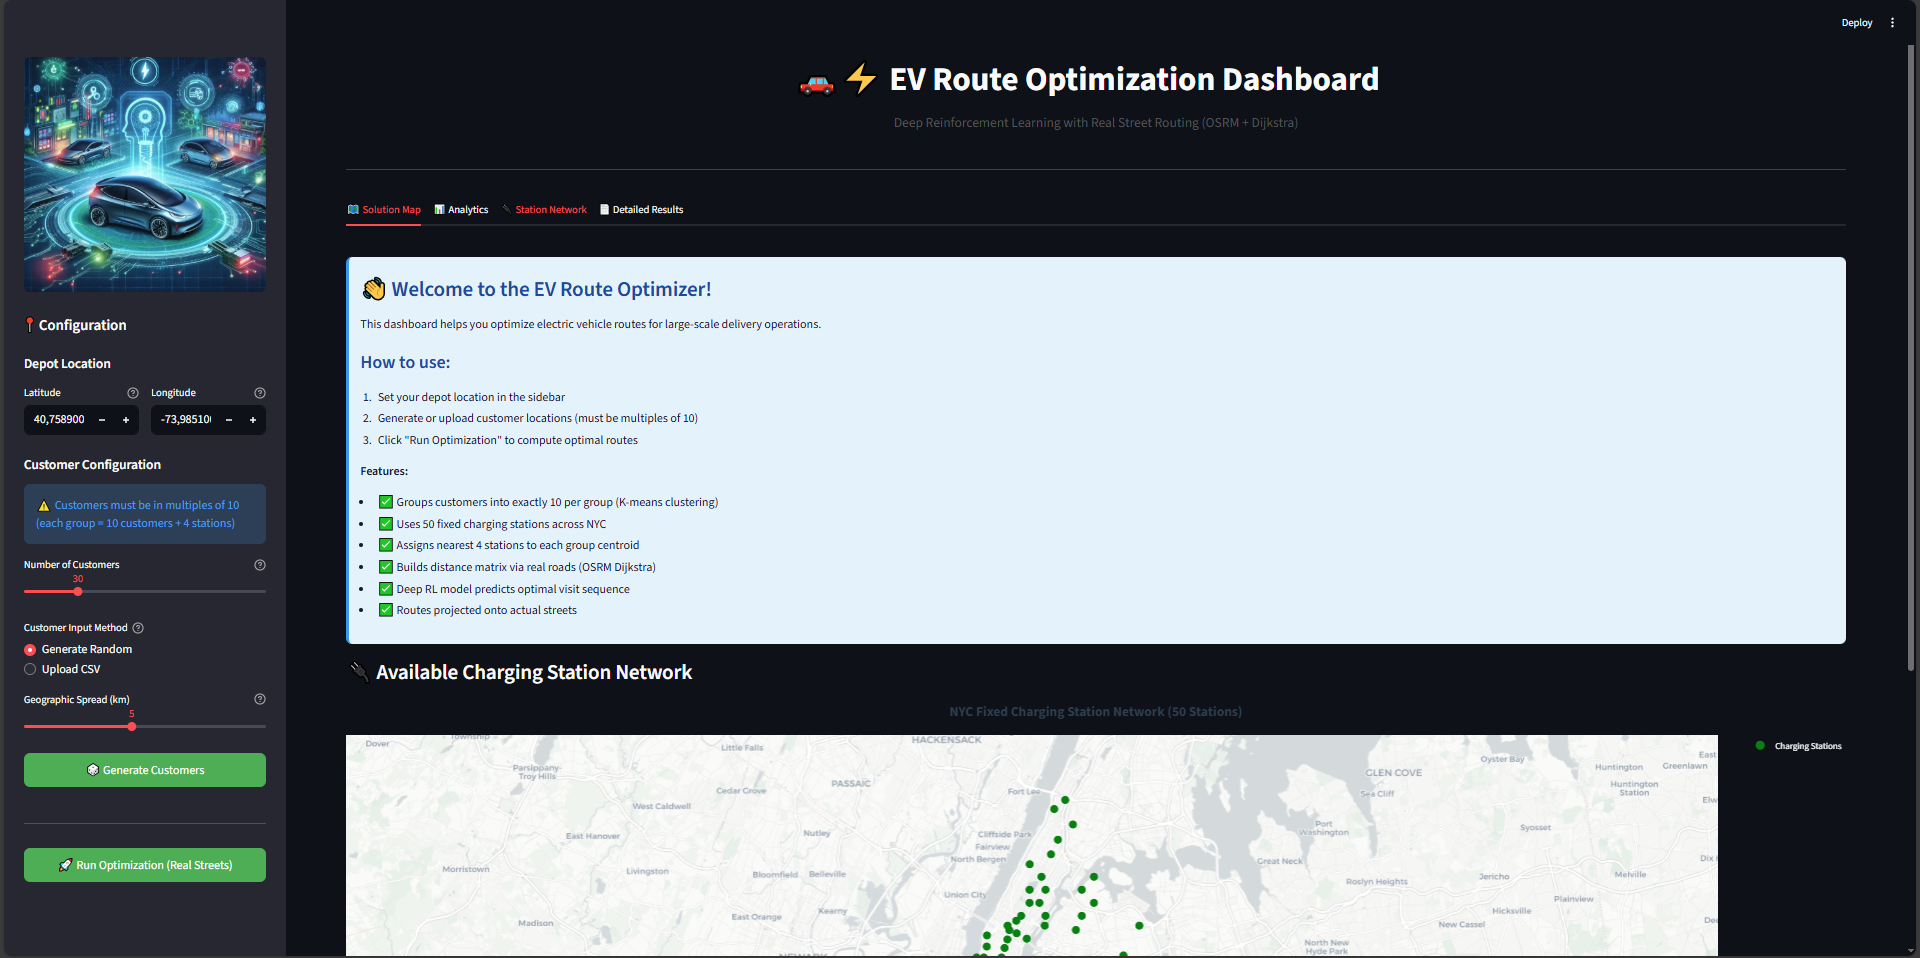
\includegraphics[width=\textwidth]{figures/main_page.PNG}\caption{Main interface}\end{subfigure}
\hfill
\begin{subfigure}{0.48\textwidth}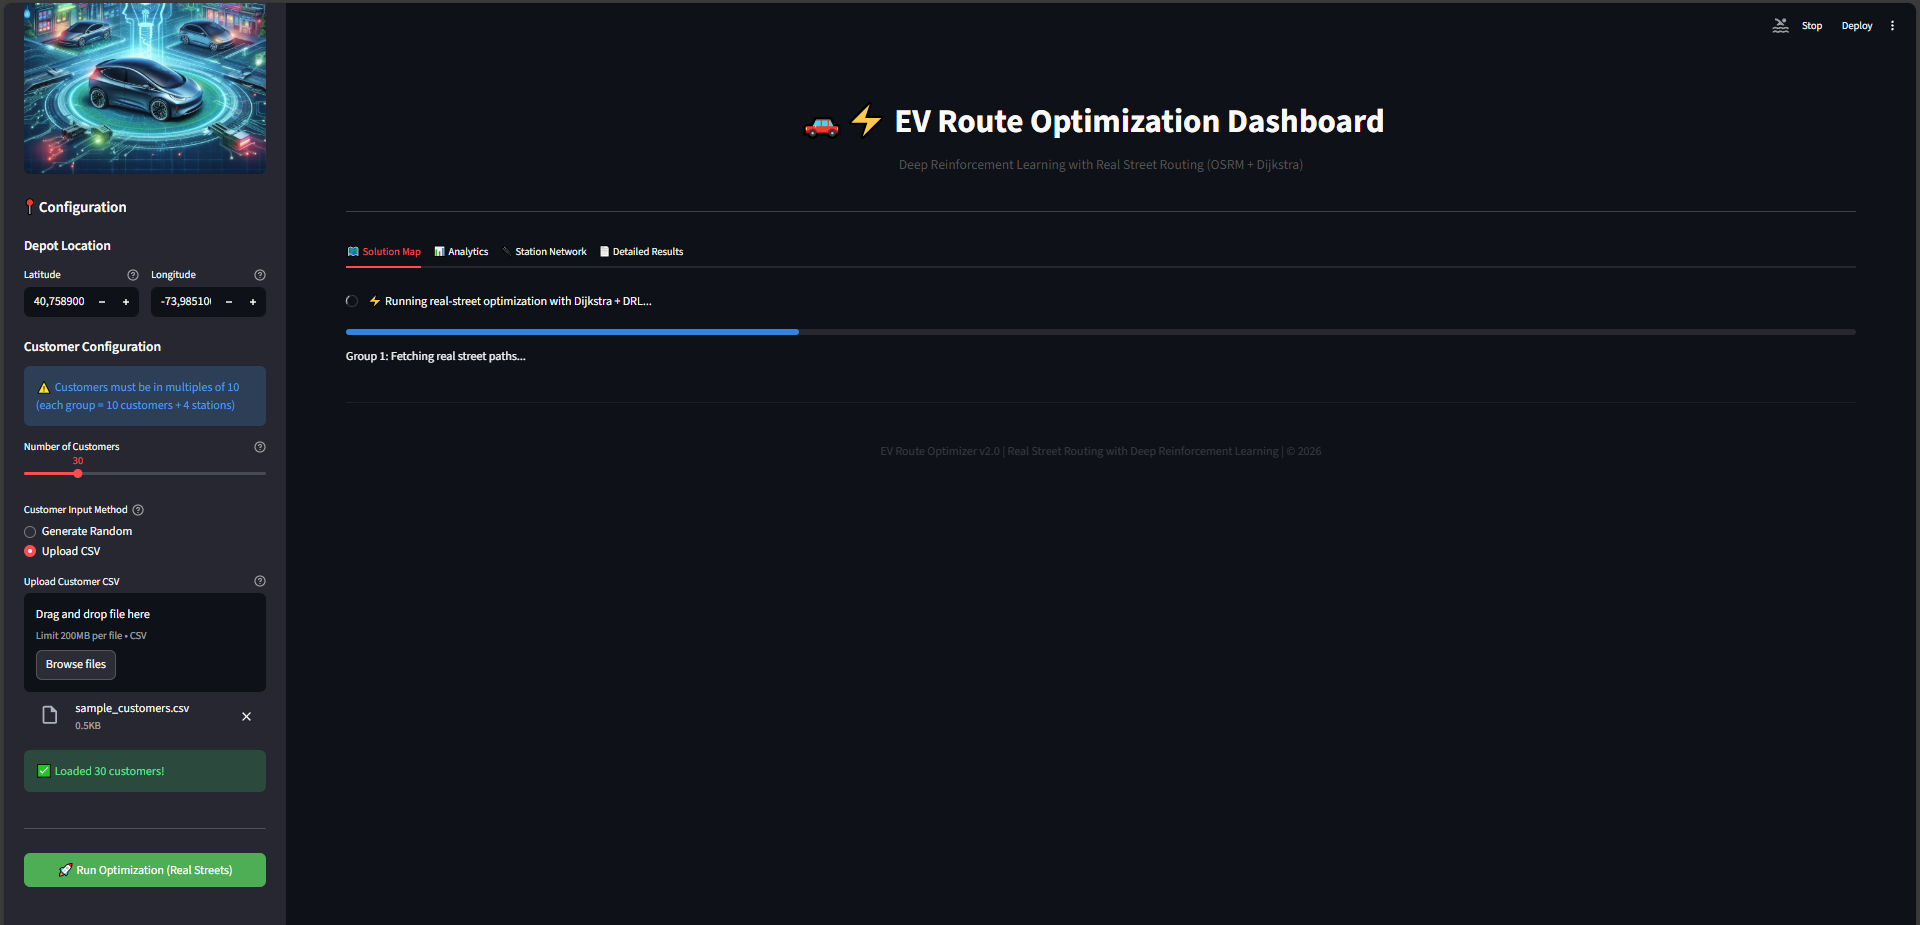
\includegraphics[width=\textwidth]{figures/inference.PNG}\caption{Inference}\end{subfigure}
\vspace{0.2cm}
\begin{subfigure}{0.48\textwidth}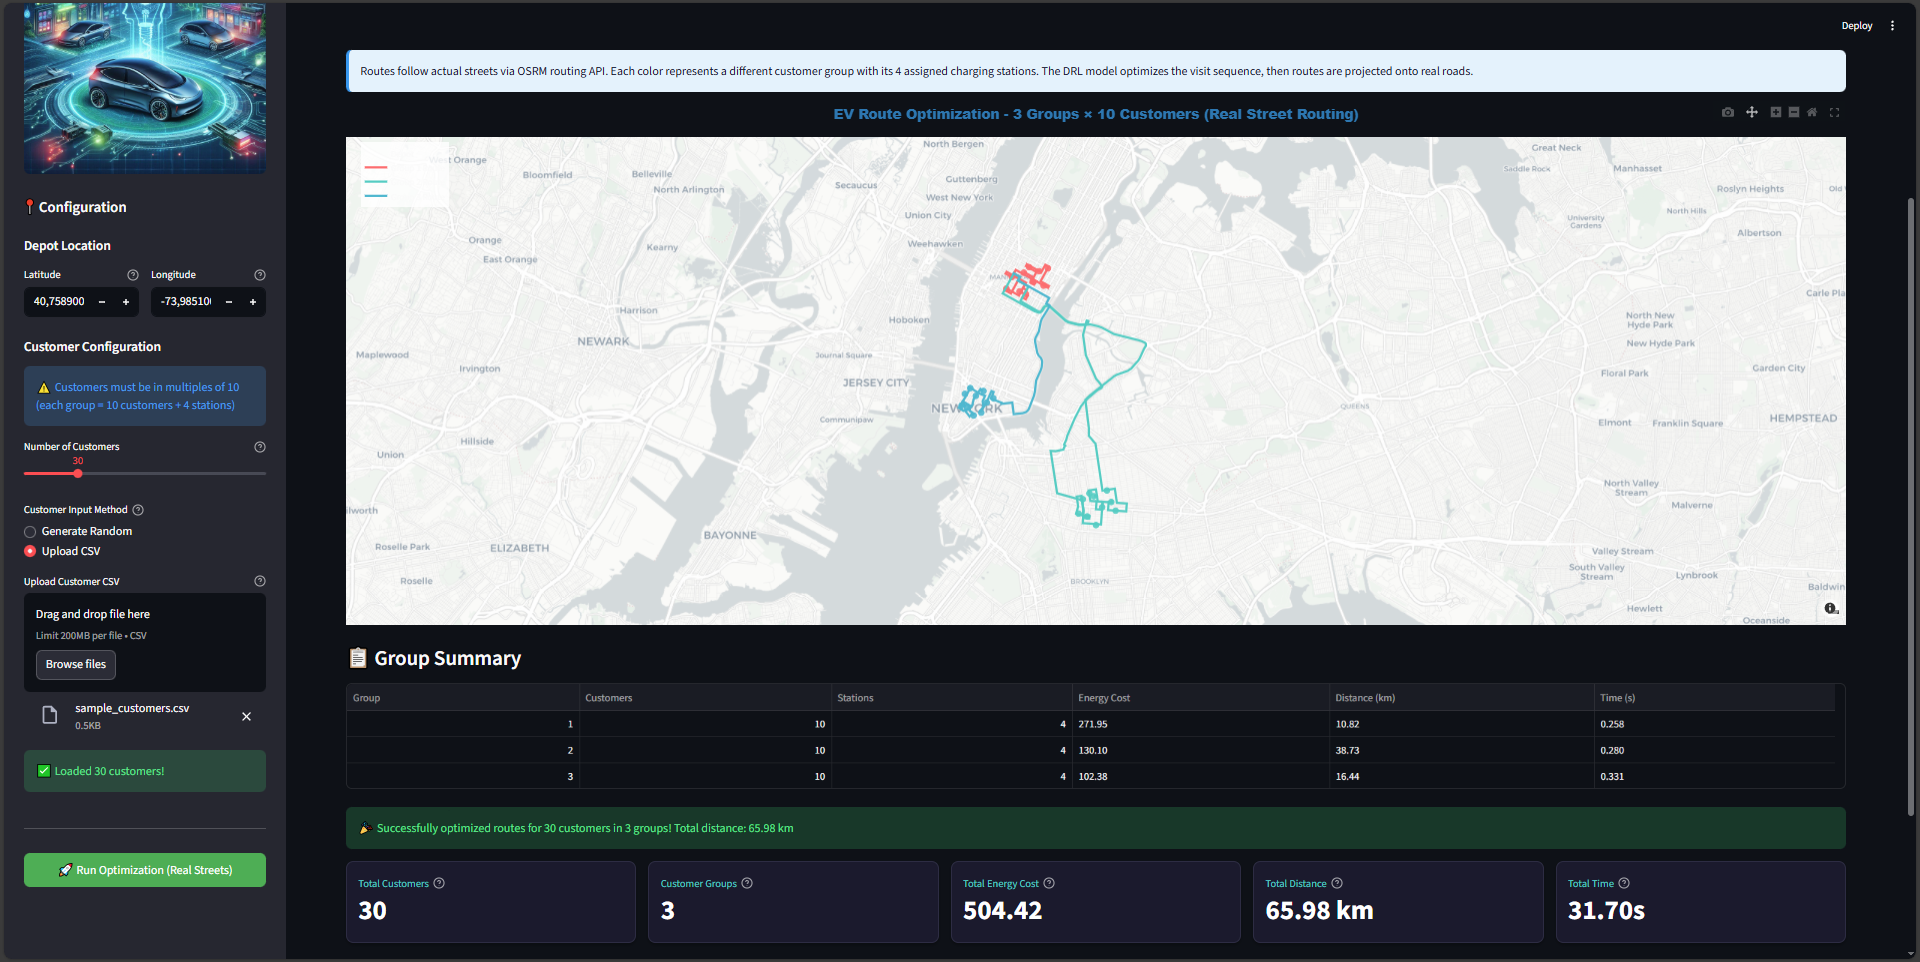
\includegraphics[width=\textwidth]{figures/result.PNG}\caption{Routes}\end{subfigure}
\hfill
\begin{subfigure}{0.48\textwidth}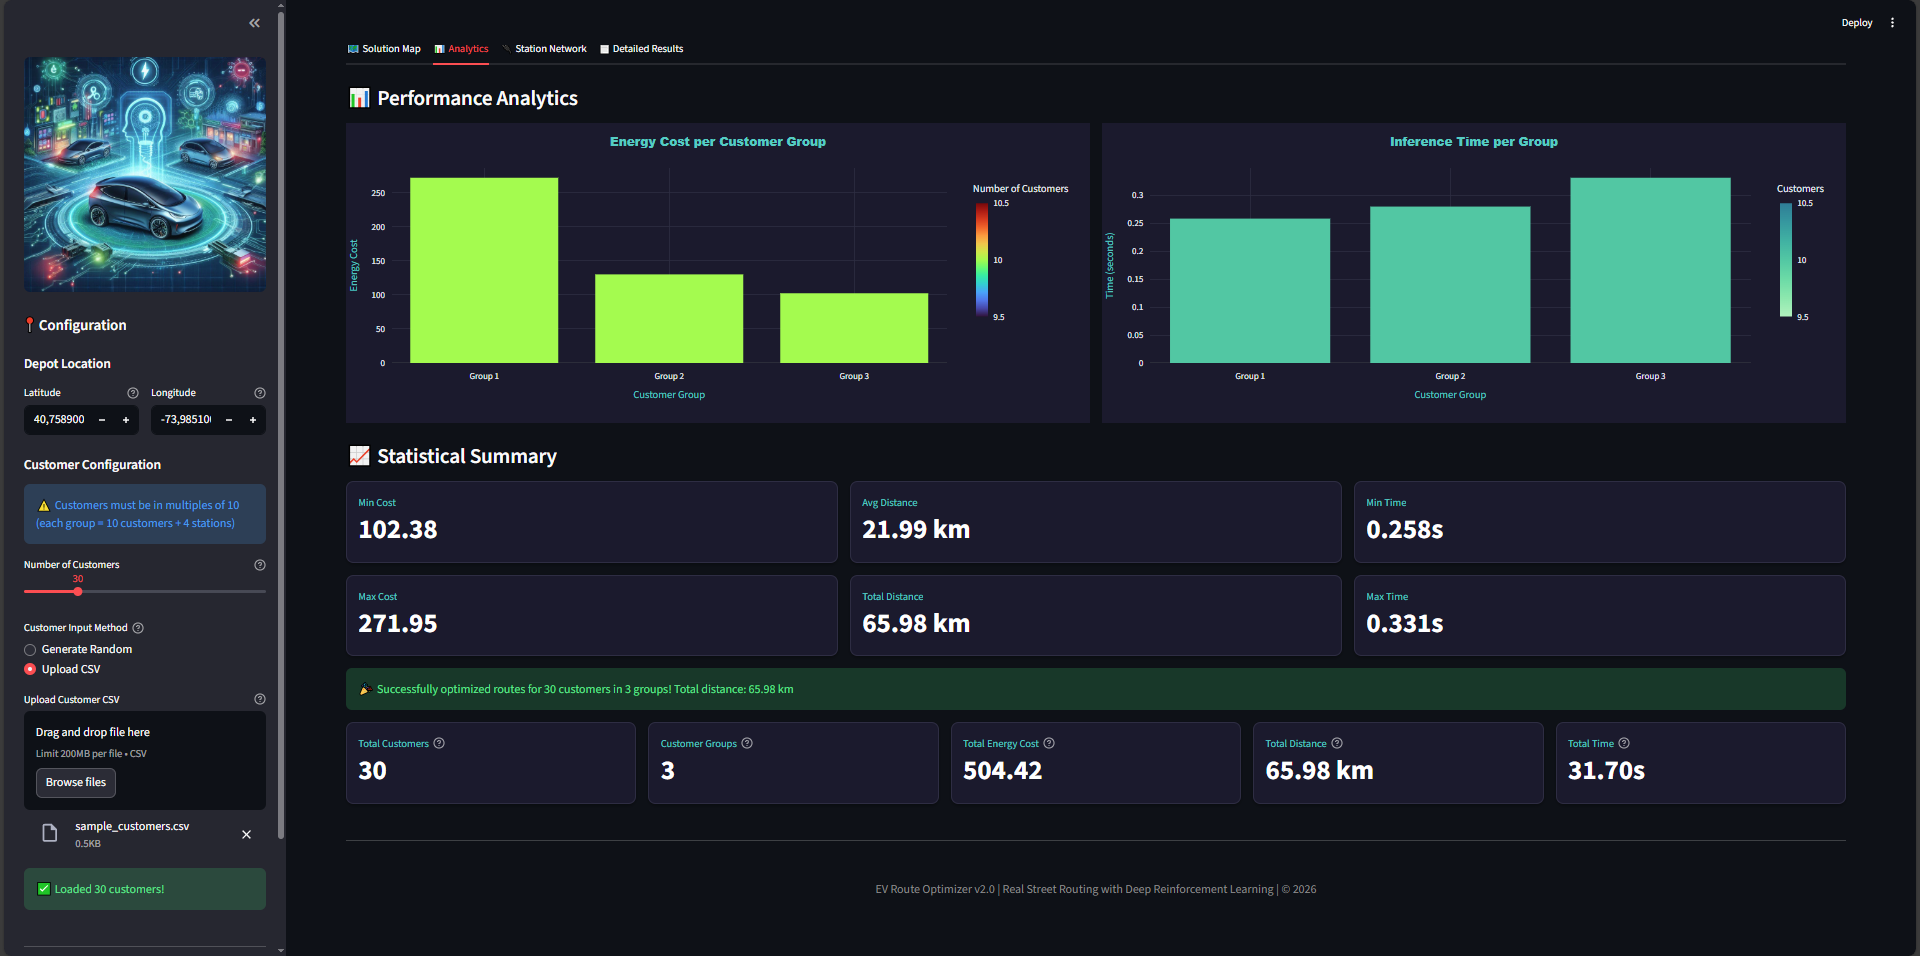
\includegraphics[width=\textwidth]{figures/analytics.PNG}\caption{Analytics}\end{subfigure}
\caption{Dashboard interfaces for EV route optimization}
\label{fig:dash}
\end{figure}

\section{Conclusion}
\subsection{Summary}
This project addressed the Energy-Minimizing Electric Vehicle Routing Problem using Deep Reinforcement Learning. Our contributions include: (1) comprehensive MILP formulation incorporating multi-trip capability, time windows, and physics-based energy consumption; (2) implementation of classical baselines for benchmarking; (3) attention-based DRL model achieving competitive performance with fast inference; (4) interactive dashboard with real-world map integration.
\subsection{Key Findings}
The DRL approach generalizes well to unseen instances after training on synthetic data. Inference time is significantly lower than iterative optimization methods. The attention mechanism effectively captures customer-to-customer relationships. Physics-based energy modeling provides realistic consumption estimates considering aerodynamics, rolling resistance, and regenerative braking.
\subsection{Future Work}
Several directions could extend this work: scaling to larger instances (50+ customers), incorporating dynamic scenarios with real-time traffic and demand updates, extending to multi-depot problems, supporting heterogeneous fleets with different EV types, and joint optimization of routing and charging schedules.

\addcontentsline{toc}{section}{References}
\begin{thebibliography}{9}
\bibitem{kool} W. Kool, H. van Hoof, M. Welling, ``Attention, Learn to Solve Routing Problems!'' \emph{ICLR}, 2019.
\bibitem{osrm} Project OSRM - Open Source Routing Machine. \url{http://project-osrm.org/}
\bibitem{ortools} Google OR-Tools. \url{https://developers.google.com/optimization}
\bibitem{cvrplib} CVRPLIB: Capacitated Vehicle Routing Problem Library. \url{http://vrp.atd-lab.inf.puc-rio.br/}
\end{thebibliography}
\end{document}